\documentclass[10pt,conference,compsocconf]{IEEEtran}
\usepackage{amsmath}
\usepackage{booktabs}
\usepackage[T1]{fontenc}
\usepackage{graphicx}
\usepackage{hyperref}
\usepackage[utf8]{inputenc}


\begin{document}
\title{AtLoc4TOPO: Adapting Attention Guided Camera Localization for the Geodetic~Engineering Laboratory (TOPO) at EPFL}

\author{
  Gerber Frédéric, El Alaoui Réda and Reding Simon\\
  \textit{Project 2, Machine Learning (CS-433), EPFL}
}

\maketitle


\begin{abstract}
This project tackles the pose estimation problem by bypassing intermediate steps. Precisely, instead of generating absolute coordinates from an image, and then using these to extract a pose, we adapt the AtLoc paper in order to get the pose directly. Additionally, we provide intermediate saliency maps, which show the most robust points of an image.
\end{abstract}


\section{Introduction}

With the wide spread of electronic devices these days, it has become increasingly important for users to locate themselves in time and space using the Global Positioning System (GPS). Indeed, additionally to being the most important clock source, GPS provides information about the position of a receiver using satellites that orbit around the Earth. Practically, this simple mechanism has many use cases, among which self-driving cars or flying drones.

However, not only is GPS vulnerable to attacks, but in remote locations like mountains, a signal may not even be available. This leads to the idea of using a different way of acquiring precise localization information. For instance, in the drone case we will focus on, two elements are necessary for good orientation: (1)~the \emph{position} in three WGS84 coordinates, and (2)~the \emph{orientation} in degrees. When bundled together, these two pieces of information are usually called a \emph{pose}.

Compared to other, more specialized sensors, cameras are low-cost and highly available nowadays, and they usually come as built-in components of drones, so it seems practical to use their images as inputs to learn poses with a machine learning model. On the high level, we want to achieve the following approximation:
\[ f(\mathrm{image})\ =\ \mathrm{pose}\ \big[\equiv (\mathrm{position}, \mathrm{orientation})\big]. \]

Researchers have already been working on camera localization in aerial contexts, but it is largely impractical to rely on previous photographs in order to train a predictor for poses in unknown locations. As a result, since the community typically trains and tests their models on real datasets, the next step consists in training  on \emph{synthetic datasets} and later evaluating them on real images. For instance, Yan \cite{yan2020oneshot} from the TOPO laboratory at EPFL achieves this in two steps: (1) create a three-dimensional absolute coordinate from a two-dimensional image, and (2) use these intermediate coordinates to output an estimate of the pose. Overall, the final accuracy is very good, since poses are at most 10 meters away from the ground truth.

Another approach is using data to directly estimate position and orientation. To make this approach more robust, attention guided techniques \cite{wang2019atloc} are used, that is, models which focus on features that are robust across many inputs. Intuitively, the network learns what is most important in the image. This paper, called AtLoc, uses \emph{saliency maps} to visualize the robust features of the input image.

Subsequently, this report will (1) describe the task we have performed in the scope of this machine learning project, (2) detail the way we adapted and ran the code, and (3) discuss the evaluation results of our method.



\section{Description of the Task}

As mentioned in the Introduction, pose estimation is ideally trained on synthetic images, while the testing and actual predictions happen on real images. Since these types of data items don't look the same, subject to weather or lighting conditions, it is interesting to benefit from the attention guided approach developed in AtLoc \cite{wang2019atloc} to focus only on the lines that matter most in an image. Therefrom, this section will go through a more precise description of the task we are addressing in our work.

\begin{figure}[hbpt]
\scriptsize
\includegraphics[width=\linewidth]{images/ONESHOTvsATLOC}
\caption{\textbf{Previous work (a) \emph{vs} AtLoc (b)}: In (a), the coordinates are generated as an intermediate step, while (b) directly estimates the pose (position, orientation) with internally a visual encoder, an attention module and a pose regressor; see \cite{wang2019atloc} for details.}
\label{fig:oneshot-atloc}
\end{figure}

\subsection{OneShot Camera Pose Estimation}

More precisely, Figure~\ref{fig:oneshot-atloc} shows a comparison between prior work and our adaptation of AtLoc for pose estimation with the TOPO datasets. In fact, Yan regresses in his work \cite{yan2020oneshot} a set of absolute coordinates from a $480\times 640\times 3$ RGB image with a deep neural network. After that, he applies a custom RANSAC solver called DSAC \cite{brachmann2018dsac} to get the final pose, \emph{i.e.} a position and an orientation.


\subsection{Attention Guided Camera Localization}

On the other hand, AtLoc internally creates attention maps that can be visualized using \emph{saliency maps}, whereby the most important features are highlighted. This construction is only an intermediate step though, so pose regression happens directly with an image once the model has been trained\footnote{The authors of the AtLoc paper have tested their method on the 7Scenes and RobotCar datasets.}. Consequently, geometrically robust features are more likely to need `attention', which is the reason why the TOPO lab is interested in this work. As a result, our work consists in the following steps: (1) run the AtLoc code as provided in its official repository, (2) adapt its dataloader and run scripts to plug some custom TOPO datasets into it, and (3) interpret/optimize the results. Finally, the ultimate goal is to find out whether AtLoc is any good in pose estimation.

% calculate saliency maps
% see if AtLoc is any good in pose estimation

%\begin{enumerate}
%    \item Try to run the code on GitHub 
%    \item Plug the TOPO dataset into AtLoc 
%    \item Get first results 
%    \item Investigate features for best predictions 
%    \item Optimize results
%\end{enumerate}

% how it fits in the TOPO research


\section{Running the Code with a New Dataset}

The AtLoc Paper shows its performance on indoor and outdoor datasets with pictures and cameras attached to a car. In those images, stable features include edges of house walls, pieces of furniture and the contour of the horizon. Moreover, unstable features which AtLoc successfully avoids in these scenes are cars, pedestrians and texture-less surfaces in general. Since our use case focuses on drones, we will have to test whether AtLoc successfully identifies other stable features in more rural environment and from different perspectives in new datasets provided by the TOPO lab at EPFL.
\subsection{The Datasets}
We have customized dataloaders for three datasets:
\begin{itemize}
    \item Comballaz Synthetic Archive;
    \item Comballaz (Air 2);
    \item EPFL (Phantom).
\end{itemize}
\begin{figure}[hbpt]
\scriptsize
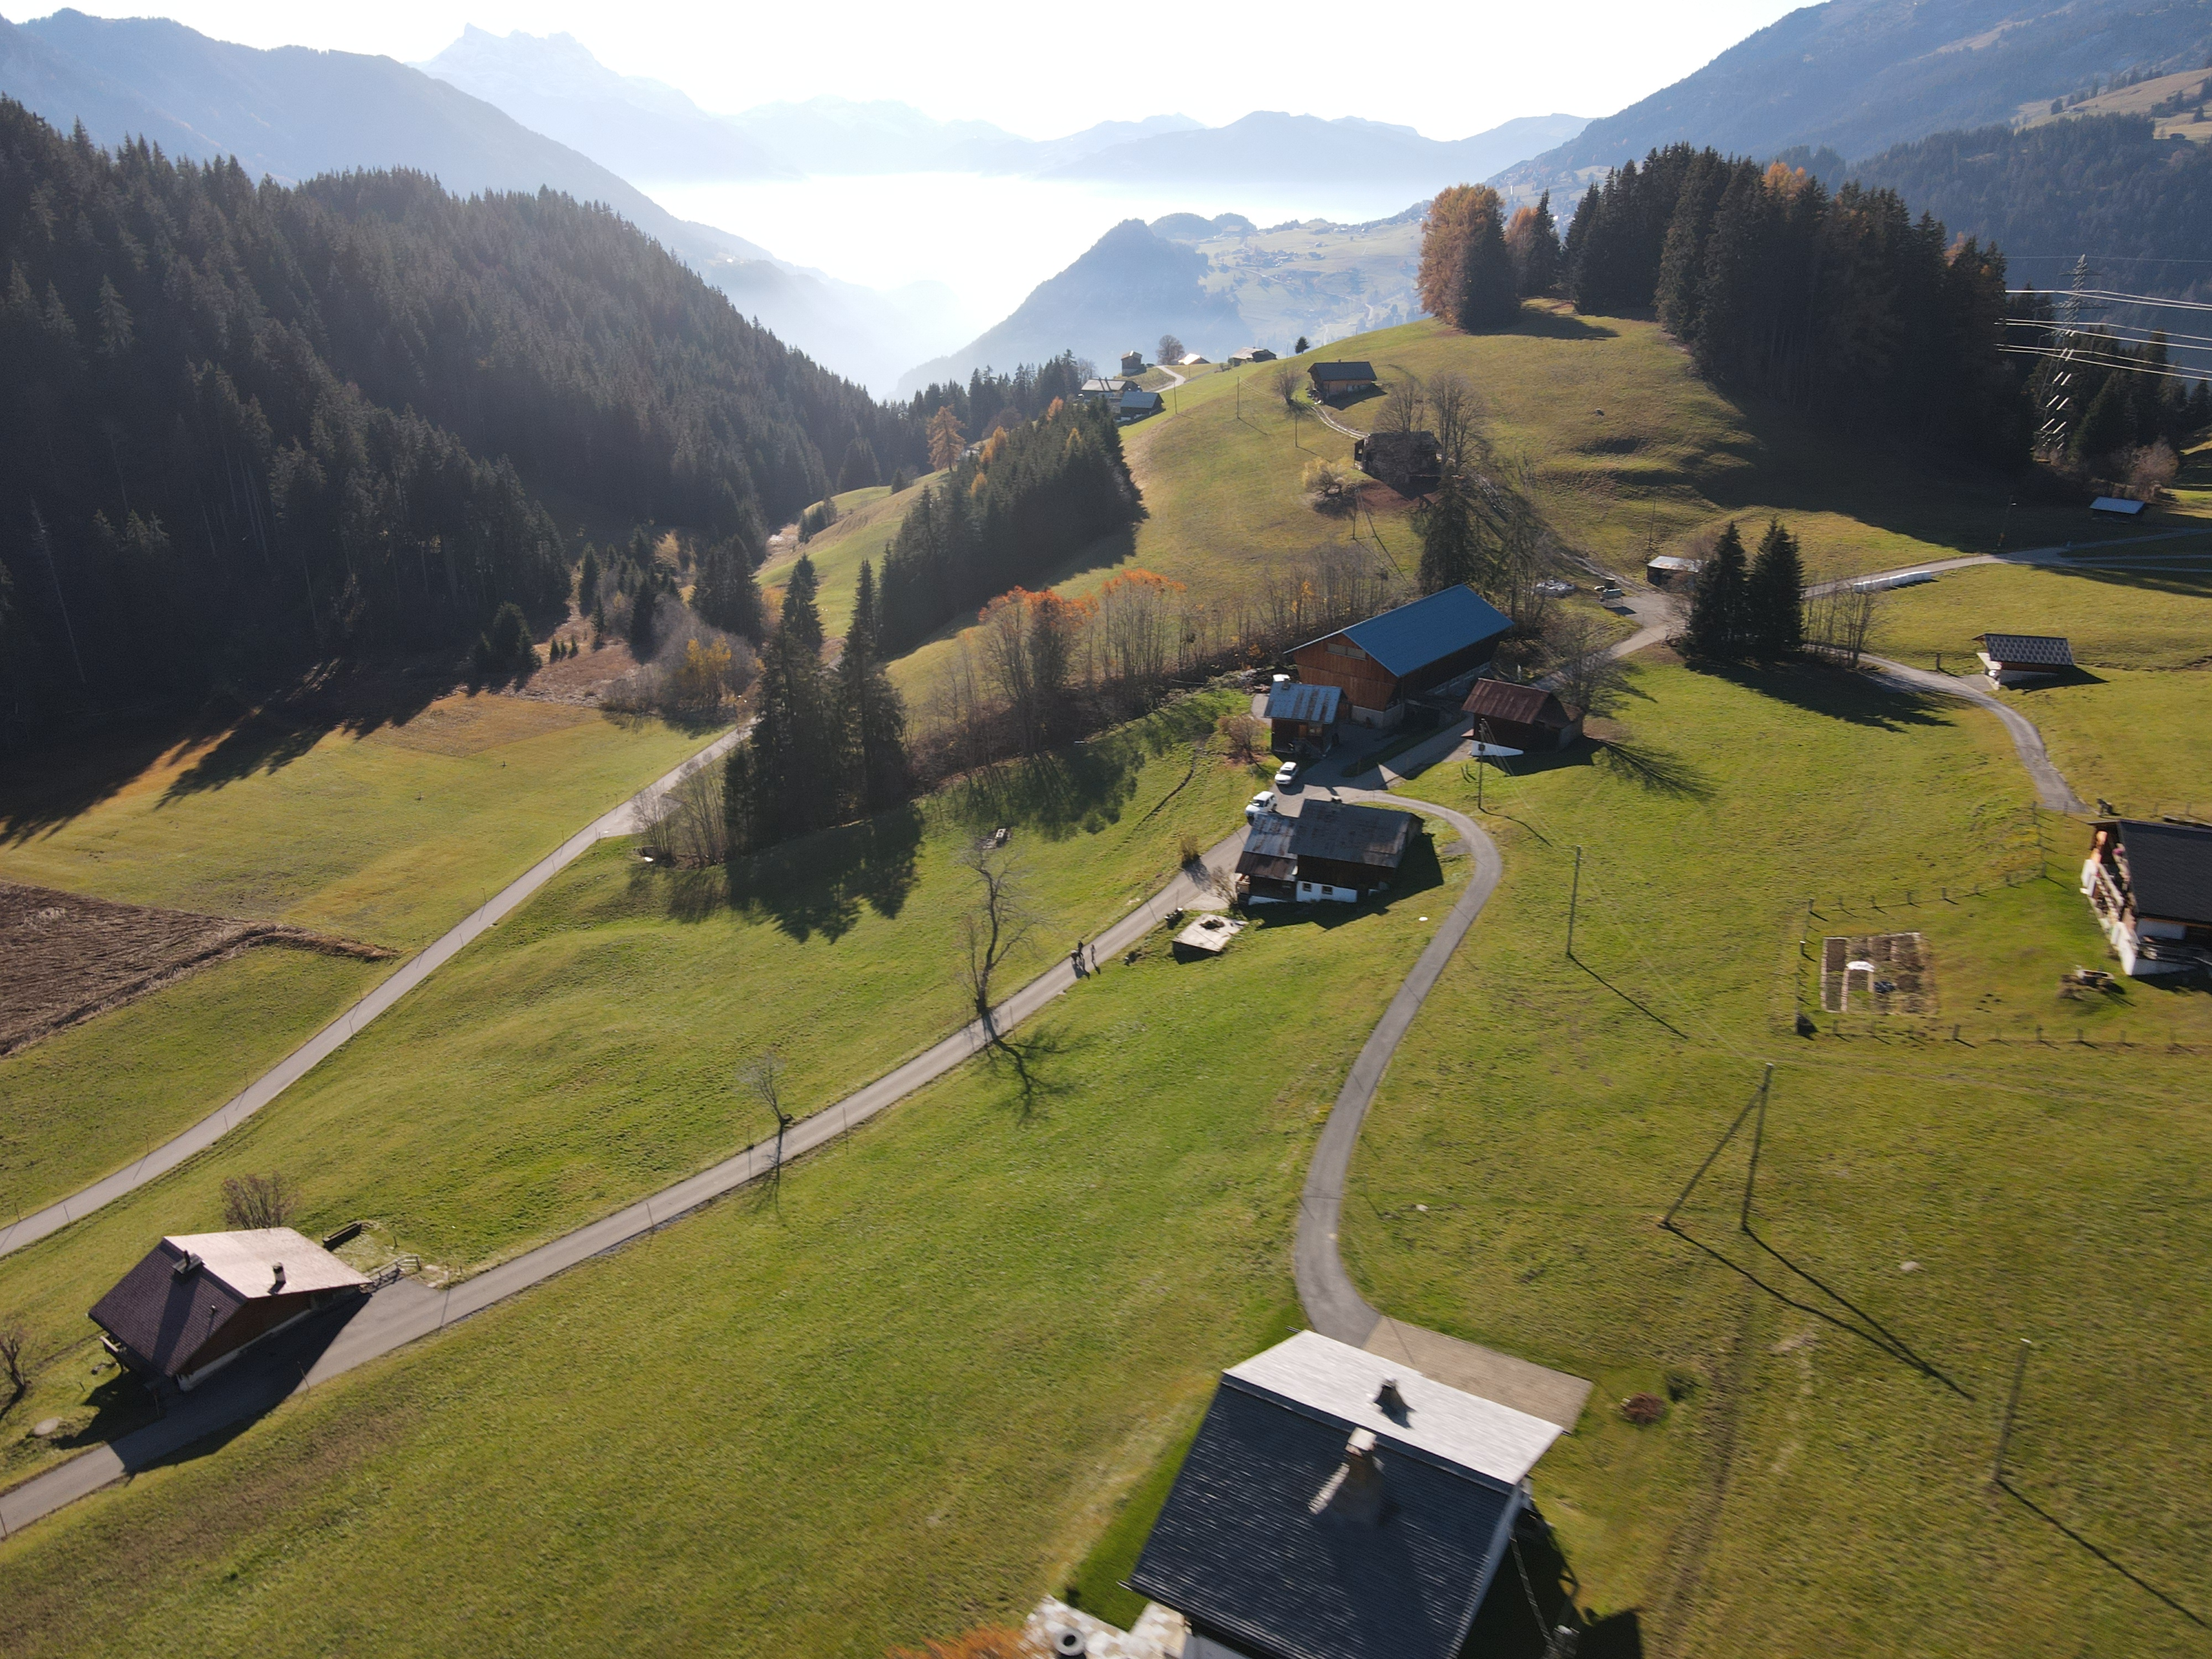
\includegraphics[width=\linewidth]{images/air_features.JPG}
\caption{\textbf{Seasons change features even in seemingly optimal weather conditions}: In addition to color changes in the whole image, there are several trees in the center of the image where the canopy is missing due to the lost leaves, revealing the texture of the ground behind it. The fog in the valley as well as the angle of the sun block additional texture in the distance: only the silhouette of the main ridgelines are visible. Observe also the larger shadows cast which are caused by the time of day but also amplified due to the season.}
\label{fig:real_seasons}
\end{figure}
\begin{figure}[hbpt]
\scriptsize
\includegraphics[width=\linewidth]{images/air2_synth.png}
\caption{\textbf{Synthetic counterpart to the real image}: We can see that evergreen and leaved trees are indistinguishable. In addition, some solid, stable features such as power lines are missing. Additionally, the better lighting pronounces the texture along the forest edge and the texture of the alps in the distance.}
\label{fig:fake_seasons}
\end{figure}

The first dataset is, as the name indicates, a large dataset of synthetically generated images, while the other two contain real images recorded on drones, combined with matching synthetic images at the exact same poses, as compared on Figures~\ref{fig:real_seasons} and~\ref{fig:fake_seasons}. Notable here is that different drones capture scenes differently: while the DJI Phantom has its camera recording close to vertically, recording features from above (top down), the Air 2 records images horizontally, capturing ridgelines and other stable features on the horizon, but in some images also a large portion of sky. Such empty spaces contain no features at all in the synthetic case, but in the real data they may contain a large amount of unstable features, like clouds, planes or the sun\ldots

Since drones move in the 3D space, we further modify the poses to better fit our use case. In particular, instead of $\text{pose}_{\text{AtLoc}} = (\text{lat},\text{long},a,b_i,c_j,d_k)$ with latitude/longitude WGS84 coordinates and quaternions, we use $\text{pose}_{\text{TOPO}} = (x,y,z,\text{pitch},\text{yaw},\text{pitch},\text{roll})$ where $x,y,z$ are ECEF coordinates derived from the WGS84 and height information provided in the datasets. This allows us to account also the error in height. We compute the distance $d$ between the target $t$ and predicted $p$ as:
$$d = \sqrt{(x_{t}-x_{p})^2 + (y_{t}-y_{p})^2 + (z_{t}-z_{p})^2}$$
using the 3D Pythagorean theorem.

\subsection{In Search of Stable Features}

Keeping the applications of drones in mind, we have to choose stable features over seasons and time of day that the mechanism can `pay attention' to:
\begin{itemize}
\item \textbf{Ridgelines}: These are perhaps the most stable features, especially when considering distinct features of the Alps of our datasets. However, they may not always be available due to cloud cover or, in the case of the Phantom dataset, completely absent due to the camera angle. It should be noted that this feature will not be extensible to other regions: in many places, mountains are too far away to be visible in plain sights, or the ridgelines not distinct enough\footnote{This is the case, for example, in the Jura mountain range.}.
\item \textbf{Buildings}: They are relatively stable, but may not always be available or distinct enough (rooftops often have similar shape and texture).
\item \textbf{Forests}: Those are stable in location but change their form during the season. It is important here that leaf trees can change the landscape significantly throughout the seasons: the missing canopy can reveal additional features such as roads and streams that would not be visible in the summer.
\item \textbf{Roads}: While in extreme conditions (during or immediately after heavy snowfall) or particular circumstances (when they are closed thus unrecognizable from the air), they tend to be a stable feature with a distinct shape. But more importantly, their texture won't change during the day as they are flat on the ground: they will be less affected by shadows.
\end{itemize}


% Explain the composition of the dataset

\subsection{Running Code on the IZAR Cluster}

Now that we are familiar with the datasets, let's dive into the actual code. Fortunately, the repository provided by the AtLoc authors\footnote{\url{https://github.com/BingCS/AtLoc}} has clear instructions regarding Python dependencies on \texttt{numpy}, \texttt{torch} and other specific modules. However, it relies on \texttt{Conda}, whereas the IZAR cluster\footnote{IZAR is a brand new cluster with 136 GPUs as part of the SCITAS resources for HPC at EPFL.} (where the TOPO datasets are stored) only supports \texttt{pip}. Therefore, we created a custom virtual environment called \texttt{atloc} containing the necessary modules.

Additionally, we wrote several batch scripts, which both unzip the datasets to temporary directories and run either training or testing on a GPU. All in all, the process of writing and debugging those scripts probably took much longer than the ten hours that were actually needed for an their execution, but it was very instructive nonetheless.

Regarding the code, each dataset\footnote{Given the time restrictions, we decided to focus on Comballaz Air and one EPFL flight from the 24th September 2020.} led to three scripts: if we take for instance Comballaz Air, we have (1) \texttt{prepare\_air}, that copies the data from the VNAV archive into our repository file system; (2) \texttt{train\_air}, whose purpose lies in offloading the lengthy model training to a GPU; and (3) \texttt{eval\_air}, in which the previously trained model is tested on a small fraction of the data. Similar scripts are available for the EPFL dataset we tested, as described in the README file\footnote{\url{https://github.com/CS-433/cs-433-project-2-eightyears}}.


\subsection{Initial Models on the TOPO Dataset}

Figure~\ref{fig:saliency-synthetic} provides a first impression from a reduced version of the Comballaz Air dataset: the attention module manages to draw more attention to stable features with texture such as the road and away from the sky, which seems promising. However, we have noticed that here and in some other images, there is also some attention drawn to unstable features in this context (\emph{e.g.} forests that change with seasons). In addition, some stable features such as ridgelines aren't that prominent.


\section{Model Evaluation}

\subsection{Performance Discussion}

In this Section, we are interested to find out how good the AtLoc-trained model performs on the Comballaz and EPFL datasets, regarding pose estimation and saliency maps.
 
\begin{figure}[hbpt]
\scriptsize
\includegraphics[width=\linewidth]{images/topo_loop_attention_atloc_11.png}
\caption{\textbf{Saliency Map Difference Before/After Training on Synthetic Image}: The first image is the original, the second represents the state at the beginning of training (output of the `visual encoder'), the third image is after 95 epochs of training (locally) using the first 210 pictures of the Comballaz Air dataset. The last image is a difference between the second and third, so it shows where training has been effective.}
\label{fig:saliency-synthetic}
\end{figure}

\begin{figure}[hbpt]
\scriptsize
\includegraphics[width=\linewidth]{images/comballaz_air_attention_AtLoc_19.png}
\caption{\textbf{Saliency Map Difference Before/After Training on Real Image}: The red channel in the last image represents the difference made by training, here, after 95 epochs.}
\label{fig:saliency-real}
\end{figure}


When comparing Figures~\ref{fig:saliency-synthetic} and~\ref{fig:saliency-real}, it becomes apparent that training has much more effect on real images: this may be partly because we have trained the model with both real and synthetic images in this case, but real images are much more influenced by specific conditions, while synthetic images are much more stable. However, it appears that the sky is considered too important, and this is also the case in other images. Nevertheless, we can observe that forests are still taken into account, but less, which is good since their appearance may vary across the seasons.

Finally, we would like to see the ridgelines gain in importance for the attention map, which is not the case here\footnote{Better training could include more epochs, which could be explored by further research. We had to clamp our experiments due to the lengthy GPU script preparation and the ten-hour long execution\ldots}. However, since quite some attention is directed towards the sky and not the rest, it still defines good contours for the mountains, which is a desirable property. % conclude...

\textbf{EPFL Phantom}: What's about the EPFL images, the data is really different. For example, we have no sky or mountain edges, and since the pictures have been taken by a Phantom drone, they are all from above. As a result, the images contain mostly edges of buildings, grass areas or gray asphalt. As can be observed on Figure~\ref{fig:saliency-epfl}, the AtLoc model seems to focus its attention on areas with grass, while it \emph{loses} the focus from buildings. 

\begin{figure}[hbpt]
\scriptsize
\includegraphics[width=0.45\linewidth]{images/AttentionMap_12.png}\hfill
\includegraphics[width=0.45\linewidth]{images/AttentionMap_18.png}
\caption{\textbf{Saliency Map Differences For EPFL Flight}: These differences correspond to the last image in Figures~\ref{fig:saliency-synthetic} and~\ref{fig:saliency-real}, \emph{i.e.} the difference made by training. In particular, the highlighted points seem to be paid \emph{less} attention to after training the model.}
\label{fig:saliency-epfl}
\end{figure}


\subsection{Results}

Moving on to more quantitative results, we summarize in the Tables on Figures~\ref{tab:unmixed} and~\ref{tab:mixed} the accuracies in different testing cases.

\begin{figure}[hbpt]
\centering
\scriptsize
\begin{tabular}{@{}lcccc@{}}
\toprule
{\bf Training}& \multicolumn{2}{c}{\textbf{Synthetic Only}} & \multicolumn{2}{c}{\textbf{Real Only}} \\
{\bf Testing} & {\bf Synthetic} & {\bf Real}& {\bf Synthetic} & {\bf Real} \\
\midrule
&\multicolumn{4}{c}{\it Comballaz Air}\\
\cmidrule{2-5}
{\bf Distance [meters]}& $51.68$ & $255147.98$  & NA & $2.04$   \\
{\bf Orientation [degrees]}& \multicolumn{2}{c}{$118.22$}  & NA & $82.27$   \\
\bottomrule
\end{tabular}
\caption{\textbf{Quantitative Results For Unmixed Training}: Medians for two possible scenarios: (1) training on synthetic (archive) data only,  and (2) training on real data.}
\label{tab:unmixed}
\end{figure}


\begin{figure}[hbpt]
\centering
\scriptsize
\begin{tabular}{@{}lcccc@{}}
\toprule
{\bf Training} & \multicolumn{2}{c}{\textbf{Both Synthetic \&{} Real}} & \multicolumn{2}{c}{\textbf{Both Synthetic \&{} Real}} \\
{\bf Testing} & {\bf Synthetic} & {\bf Real} & {\bf Synthetic} & {\bf Real} \\
\midrule
&\multicolumn{2}{c}{\it Comballaz Air}&\multicolumn{2}{c}{\it EPFL 2020-09-24}\\
\cmidrule{2-3} \cmidrule{4-5}
{\bf Distance [meters]}& $69.74$ & $29094.23$ & $24.33$ & $21724.34$  \\
{\bf Orientation [degrees]}& \multicolumn{2}{c}{$144.80$} & \multicolumn{2}{c}{$110.76$}    \\
\bottomrule
\end{tabular}
\caption{\textbf{Quantitative Results for Mixed Training}: Medians for training on both real and synthetic images, where we're mostly interested in the results for real data, given the drone use case.}
\label{tab:mixed}
\end{figure}

In these Tables, we observe that when training on both types of images, synthetic predictions are much better, while real data suffers from large inaccuracies. This is probably due to the small portion of real images with respect to the huge amount of synthetic data that can be generated.

Moreover, when training on 30'000 synthetic images from the Comballaz Archive, the synthetic accuracy is slightly better than with mixed training, but not perfect either, probably since the testing images are taken at different poses. Additionally, the real accuracies drop as expected, since there are no real images in the training set.

This seems to imply that, at least with only 100 epochs, AtLoc is not able to extract common attention maps for real and synthetic images. Also, the split between real and fake images matters a lot, but it takes time to generate as many real images than there are fake ones. 

So unfortunately, extrapolating to the real data does not seem so promising, at least in the Comballaz (Air) and EPFL (2020-09-24) datasets illustrated here. However, testing on real data when the model has been trained by real data yields very good accuracy, which seems nice, but requires that the drones only be put in `known' areas, that is, locations for which PhD students from TOPO have manually created images.




\subsection{Further Improvement}

In order to have a closer match between real and synthetic data, the general idea was to have similar saliency maps, so that the attention is focused on the same features. To achieve this goal better than in this work, it should be possible to generate data, for instance by adding gray overlays to simulate clouds on synthetic landscapes, or by changing the colors from green to white to create a snow effect.

Some other ideas, as proposed by the TOPO lab, would be to use GANs to generate some (fake) real images to train from; or to dummify the images in order to keep only a low level of detail including the most important shapes.

\section{Conclusion}
To conclude, our end-to-end AtLoc network seems to produce more accurate results\footnote{But such networks have other drawbacks, like behaving as black-boxes.} than two-step networks as in \cite{yan2020oneshot}, and our use case is no different. However, while we have had success in training Atloc on new datasets, either real or synthetic, we were unable to produce meaningful results using mixed training sets. We suspect that the chasm between the two datasets is currently too large but we believe that there is indeed potential to use data augmentation on the synthetic images as well as some preprocessing on the real images to make the two datasets more alike.

%End-to-end network vs two-step network
%end to end like atloc usually a bit better, but they may appear as a black box, a bit like neural networks...




% References may be on a fifth page
\section*{Acknowledgements}
The authors thank Iordan Doytchinov for his supervision and helpful suggestions during our work, and Jiannong Fang for his patient support when debugging our scripts for GPUs. Also, thanks a lot to the whole TOPO team, in particular Qi Yan for his previous work and Théophile Schenker for providing the dataset on IZAR.



\nocite{silva2020venv}
\nocite{brachmann2018dsac}
\nocite{rezzonico2020fs}
\nocite{rezzonico2020faq}
\nocite{varini2020tensorflow}

\bibliographystyle{IEEEtran}
\bibliography{literature}


% \subsection{Figures and Tables}

\end{document}
